\documentclass{beamer}

%STYLE
\mode<presentation>{
\usetheme{CambridgeUS}
\usecolortheme{dolphin}
}

%PACKAGES
\usepackage[utf8]{inputenc}
\usepackage[german]{babel}
\usepackage[T1]{fontenc}
\usepackage{amsmath}
\usepackage{amsfonts}
\usepackage{amssymb}
\usepackage{graphicx}
\usepackage{booktabs}
\usepackage{color}
\usepackage{hyperref}
\usepackage{textcomp}
%\usepackage{transparent}
\graphicspath{{images/}}
\beamertemplatenavigationsymbolsempty

%ECKDATEN
\author[F. Rohkrähmer]{Frederik Rohkrähmer}
\title[Fakultät für Informatik]{Multi-Target Regression zur Approximation der Spielphysik von Rocket League}
\date{8. September 2022}
\institute[Lehrstuhl 11]{TU Dortmund}

\begin{document}

%----------------------------------------------------
%START
%----------------------------------------------------

\begin{frame}
\titlepage
\end{frame}

\begin{frame}
\frametitle{Inhalt}
\tableofcontents
\end{frame}

 \section{Motivation}
\begin{frame}
\frametitle{Rocket League}
\begin{minipage}[c]{0.5\textwidth}
\begin{itemize}
\item Autofußball mit Raketenantrieb
\item 2015 veröffentlicht von Psyonix
\item Seit 2019 im Besitz von Epic Games
\item Entwickelt in Unreal Engine 3
\end{itemize}
\end{minipage}
\begin{minipage}[c]{0.48\textwidth}

\includegraphics[width=\textwidth]{Rocket_League_logo.jpg}
 %https://de.wikipedia.org/wiki/Datei:Rocket_League_coverart.jpg
\end{minipage}
\end{frame}


 \begin{frame}
 \frametitle{Spielprinzip}
\begin{minipage}[c]{0.3\textwidth}
  \begin{itemize}
   \item Fußball mit Autos
   \item 1vs1 bis 4vs4
   \item Raketenantrieb
   \item (Doppel-)Sprünge
   \item Rollen
   \item Wand fahren
  \end{itemize}
\end{minipage}
\begin{minipage}[c]{0.68\textwidth}
 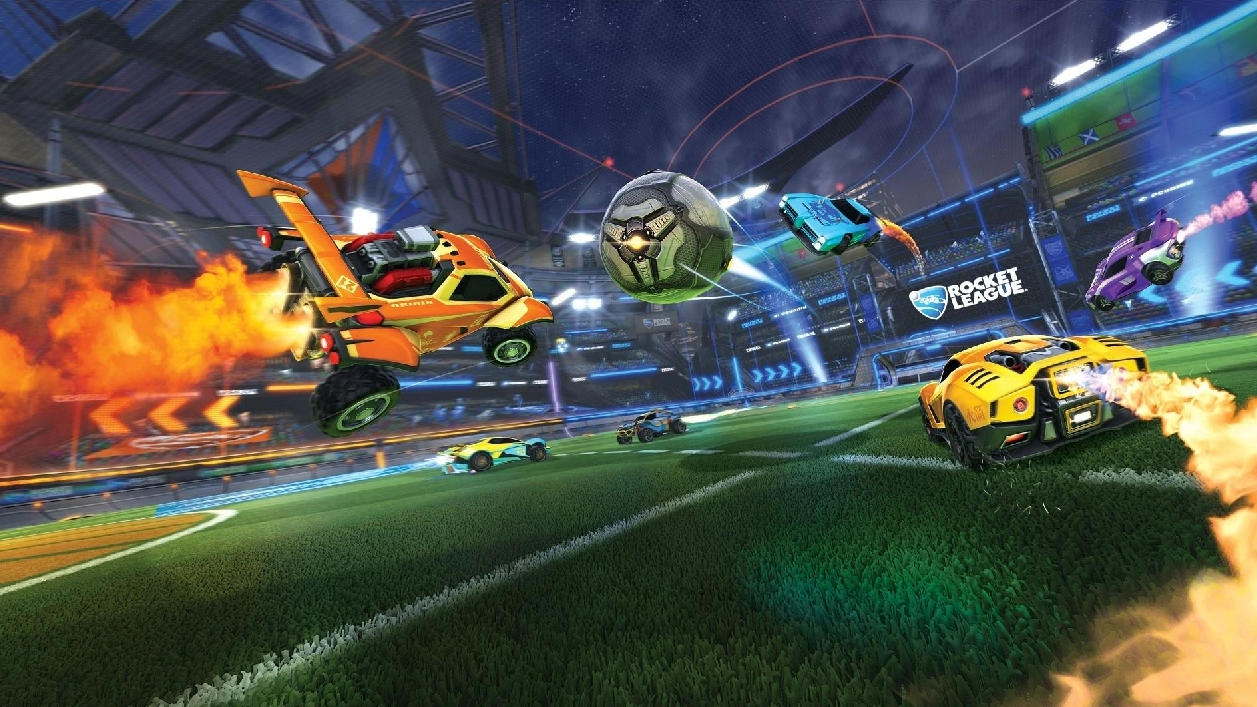
\includegraphics[width=\textwidth]{rocket_action.png}
 %https://scufgaming.com/de/gaming/rocket-league
\end{minipage}
 \end{frame}

 \begin{frame}
 \frametitle{Projektgruppe 642}
 \begin{minipage}[c]{0.5\textwidth}
  \begin{itemize}
   \item Verteiltes Deep Reinforcement Learning zum Trainieren von Game AI in Rocket League
   \item Training in Unity-Reimplementation
   \item Reverse Engineering
   \item Sim-to-Sim Transfer
   \item Paper veröffentlicht
   \item Sim-to-Sim Striker schießt nur 75\% der Tore
  \end{itemize}
  \end{minipage}
\begin{minipage}[c]{0.48\textwidth}
 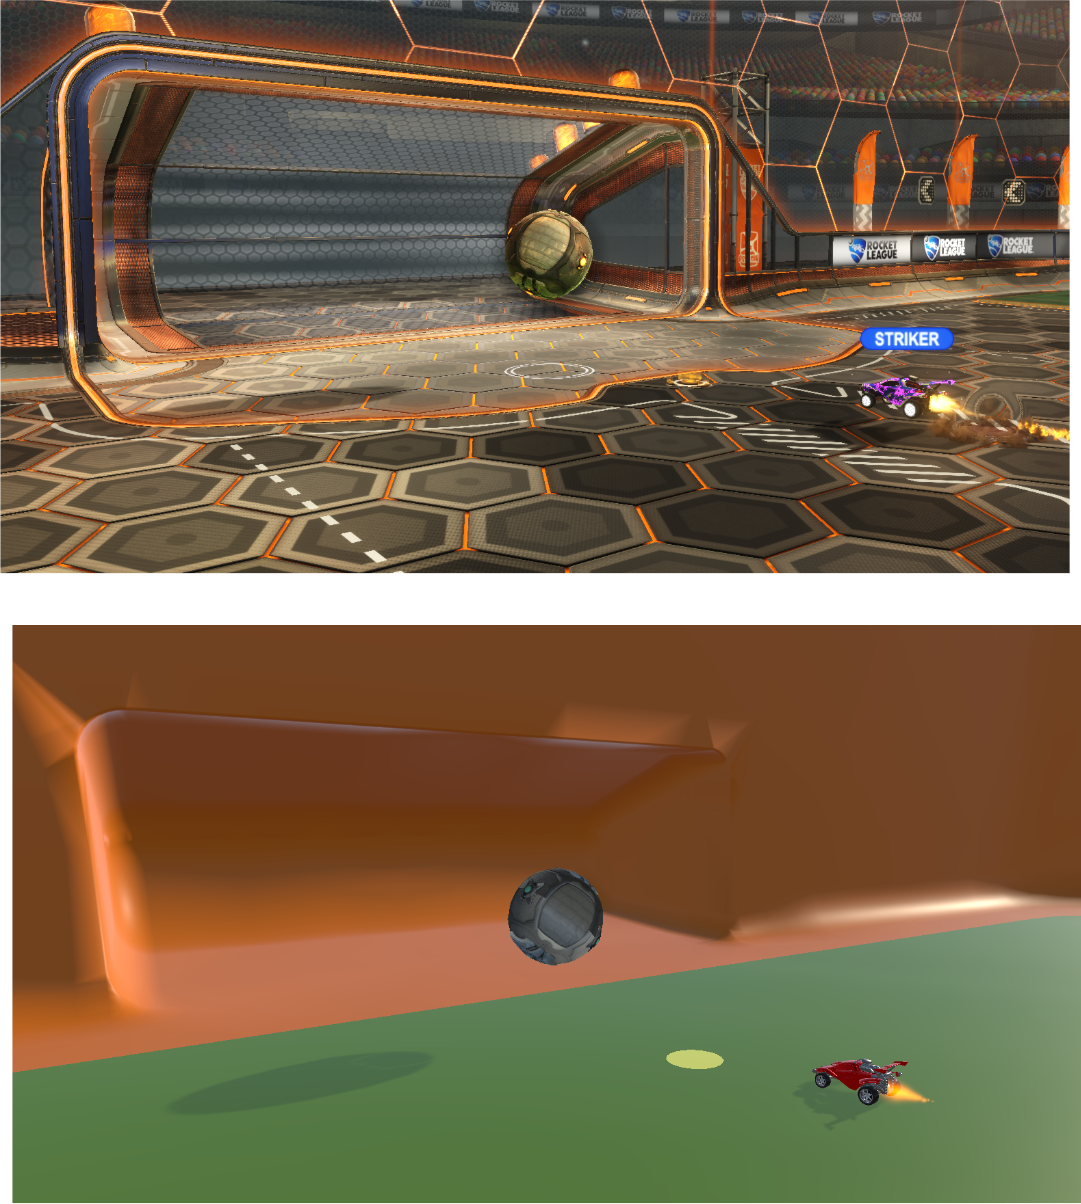
\includegraphics[width=\textwidth]{robo_vergleich.png}
 %https://arxiv.org/abs/2205.05061
\end{minipage}
 \end{frame}


 \section{Ziel}
\begin{frame}
 \frametitle{Idee}
  \begin{itemize}
   \item Sim-to-Sim Idee vielversprechend, aber
   \item Unity Implementierung nicht gut genug!
   \item Neuer Ansatz:
   \item Supervised Learning statt Reverse Engineering
  \end{itemize}
 \begin{block}{Problemstellung}
  Gegeben ein Spielzustand und ein Input, bestimme den Spielzustand des nächsten Frames so wie er in Rocket League folgen würde.
 \end{block}
  \begin{block}{Ziel}
  Erstelle ein Multi-Target Regressionsmodell, welches dieses Problem löst.
 \end{block}
 \end{frame}

\begin{frame}
 \frametitle{Multi-Target Regression}
  \begin{itemize}
   \item Klassifikation: Diskreter Output
   \item Regression: Kontinuierlicher Output
   \item Spielzustand enthält mehrere kontinuierliche Größen (Targets)
   \item Position, Geschwindigkeit, Rotation, Winkelgeschwindigkeit
   \item Vorhersage mehrerer kontinuierlicher abhängiger Variablen:
   \item Multi-Target Regression
  \end{itemize}
 \end{frame}

\begin{frame}
 \frametitle{Multi-Target Regression}
  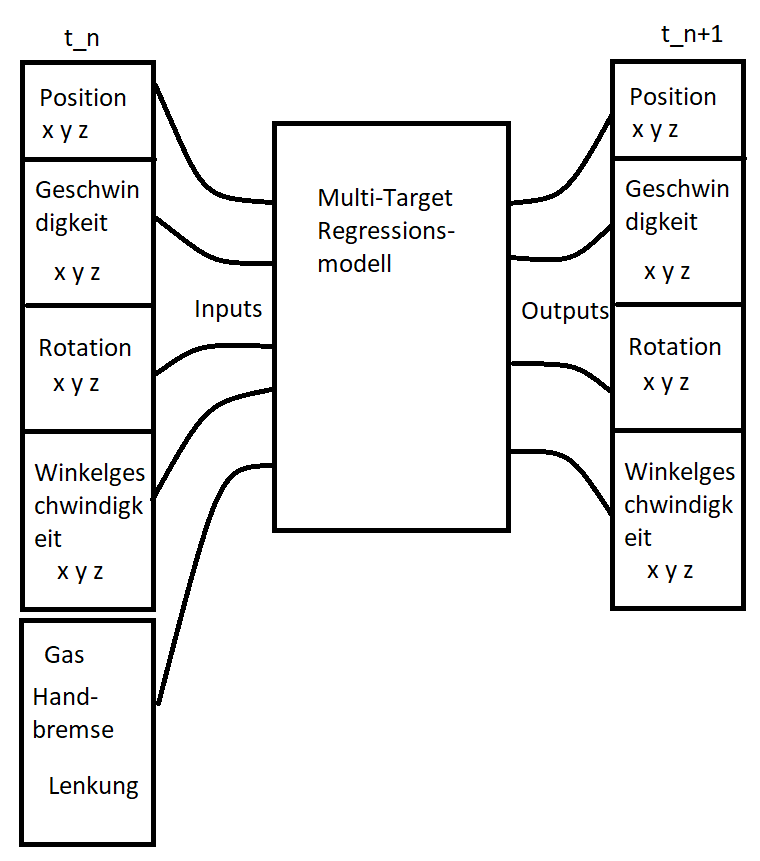
\includegraphics[height = 0.9\textheight]{MTR.png}
 \end{frame}

 \section{Datenbeschaffung}
\begin{frame}
 \frametitle{Datenbeschaffung}
  \begin{itemize}
   \item Benötigt:
   \item Aufeinanderfolgende Spielzustände
   \item mit annotierten getätigten Inputs
   \item die möglichst viele verschiedene Spielsituationen abdecken
   \item \textbf{So einen Datensatz gibt es \textit{noch} nicht!}
  \end{itemize}
 \end{frame}

 \begin{frame}
 \frametitle{Datengenerierung}
 \begin{minipage}[c]{0.7\textwidth}
  \begin{itemize}
   \item Mehrere Möglichkeiten Spielzustände auszulesen:
   \item RLBot
   \item RLGym
   \item BakkesMod
  \end{itemize}
  \end{minipage}
\begin{minipage}[c]{0.28\textwidth}
 \begin{minipage}[c]{0.33\textheight}
  
\includegraphics[width=\textwidth]{RLBot.png}
  %https://rlbot.org/
 \end{minipage}
 \begin{minipage}[c]{0.33\textheight}
  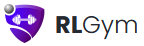
\includegraphics[width=\textwidth]{rlgym.png}
 %https://rlgym.org/
 \end{minipage}
 \begin{minipage}[c]{0.15\textheight}
  
\includegraphics[width=\textwidth]{BakkesMod.png}
  %%https://bakkesmod.fandom.com/wiki/BakkesMod_Wiki
 \end{minipage}
\end{minipage}
 \end{frame}
%https://bakkesmod.fandom.com/wiki/BakkesMod_Wiki

 \begin{frame}
 \frametitle{Spielerinputs neu simulieren}
\begin{itemize}
 \item RLGym am praktikabelsten
 \item Beschleunigbar
 \item Parallelisierbar
 \item Aber nur Windows
 \item Vorgehen:
 \item In jedem Frame Input über RLGym ausführen lassen
 \item Spielzustand aufzeichnen
\end{itemize}
 \end{frame}

 \begin{frame}
 \frametitle{Spielerinputs generieren}
\begin{itemize}
 \item Inputsequenzen benötigt die die Anforderungen erfüllen
 \item Händisch erstellen zu aufwändig
 \item Eigene Inputs aufzeichnen auch zu aufwändig
 \item Lösung:
 \item Inputs aus Replays
\end{itemize}
 \end{frame}

 \begin{frame}
 \frametitle{Rocket League Replays}
\begin{itemize}
 \item Komprimierte Datei die Spielverlauf speichert (.replay)
 \item Replays speichern KEINE Inputs
 \item Aber:
 \item Inputs lassen sich emulieren
 \item \url{https://github.com/oxrock/TrainingDataExtractor}
 \item Replays massenhaft online erhältlich z.B. auf
 \item \url{https://ballchasing.com}
\end{itemize}
 \end{frame}

 \begin{frame}
 \frametitle{Inputsequenzen aufbereiten}
\begin{itemize}
 \item Replays speichern Spielzustände mit ca. 25fps
 \item Rocket League läuft mit 120fps
 \item Replays in mehrere Sequenzen zerteilen
 \item Beginn: Anstoß, Ende: Tor
 \item 25fps Sequenzen zu 120fps interpolieren
 \item Mehrere Möglichkeiten
\end{itemize}
 \end{frame}

 \section{Training}

 \begin{frame}
 \frametitle{Beschaffenheit des Datensatzes}
  \begin{itemize}
   \item Zunächst nur 1vs1 Spiele betrachten
   \item Spielzustand ist nicht gedächtnislos!
   \item Sprungverhalten von versteckten Variablen abhängig
   \item Daher:
   \item Multi-Target Regressionsmodell mit Gedächtnis wählen
   \item Geeignet:
   \item Long Short Term Memory (LSTM)
  \end{itemize}
 \end{frame}


 \begin{frame}
 \frametitle{Long Short Term Memory}
 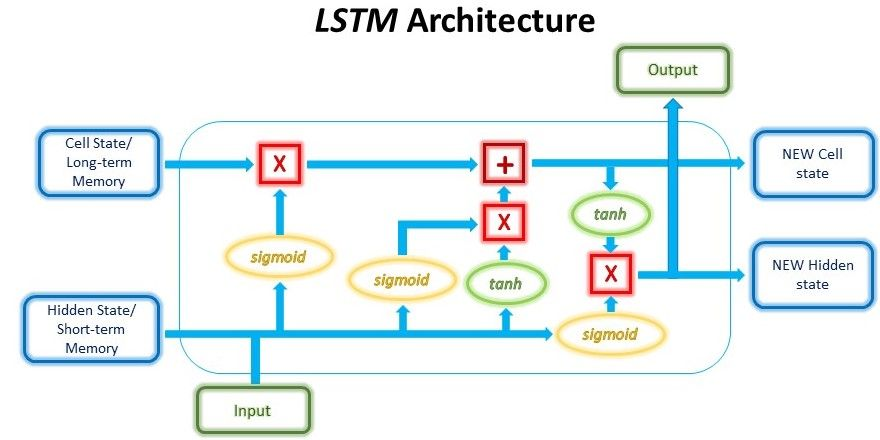
\includegraphics[width=\textwidth]{LSTM.JPG}
  %https://blog.floydhub.com/long-short-term-memory-from-zero-to-hero-with-pytorch/
 \end{frame}

 \begin{frame}
 \frametitle{Long Short Term Memory}
 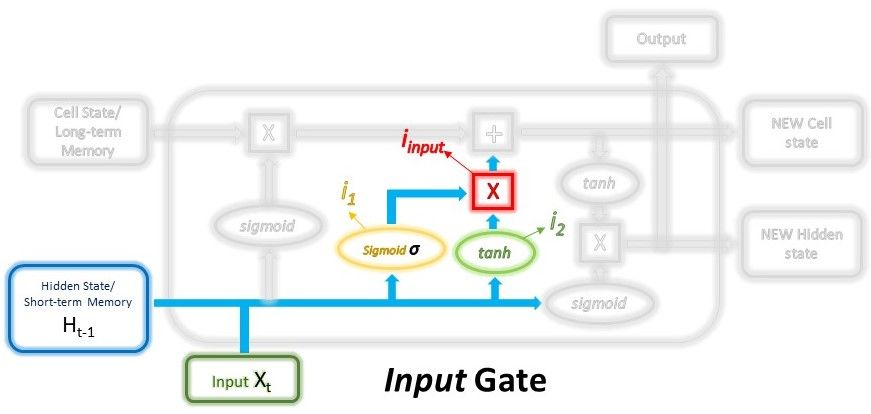
\includegraphics[width=\textwidth]{InputGate.JPG}
  %https://blog.floydhub.com/long-short-term-memory-from-zero-to-hero-with-pytorch/
 \end{frame}

 \begin{frame}
 \frametitle{Long Short Term Memory}
 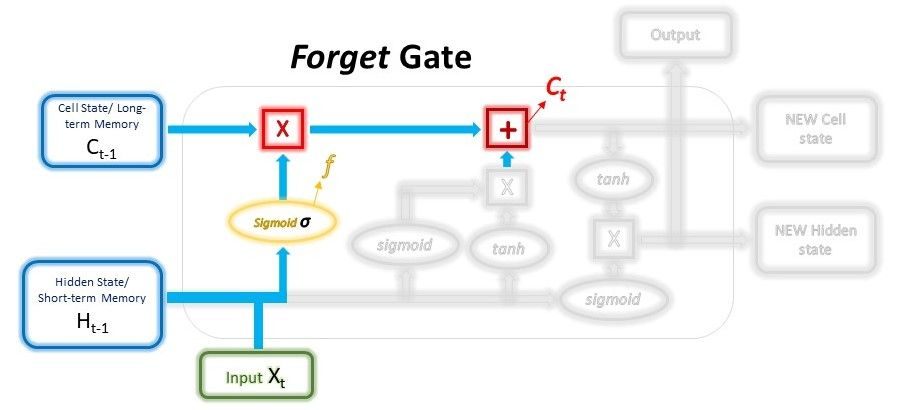
\includegraphics[width=\textwidth]{ForgetGate.JPG}
  %https://blog.floydhub.com/long-short-term-memory-from-zero-to-hero-with-pytorch/
 \end{frame}

 \begin{frame}
 \frametitle{Long Short Term Memory}
 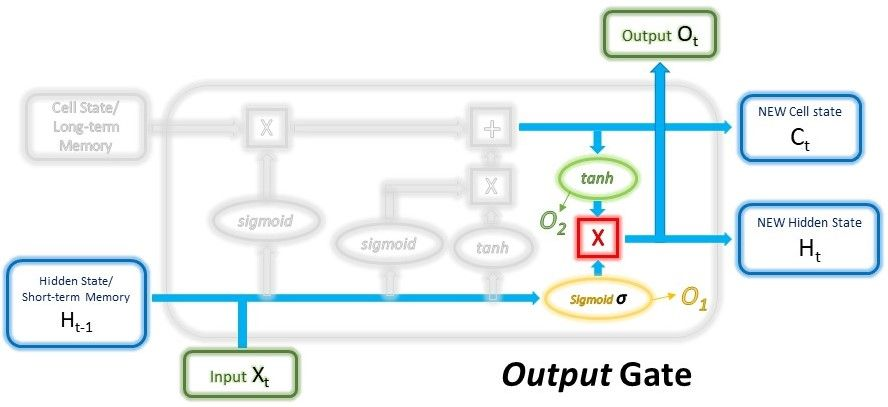
\includegraphics[width=\textwidth]{OutputGate.JPG}
  %https://blog.floydhub.com/long-short-term-memory-from-zero-to-hero-with-pytorch/
 \end{frame}

 \begin{frame}
 \frametitle{Zusammenfassung}
  \begin{itemize}
   \item .replay Dateien besorgen
   \item Emulierte Inputs generieren
   \item Auf 120 fps interpolieren
   \item Mit RLGym in Rocket League ausführen
   \item Spielzustände aufzeichnen
   \item LSTM trainieren
  \end{itemize}
 \end{frame}

  \begin{frame}
 \frametitle{Ausblick}
  \begin{itemize}
   \item Wenns gut läuft:
   \item Erweitern auf 2v2, 3v3, 4v4
   \item Agenten mit dem Modell trainieren lassen
  \end{itemize}
 \end{frame}

\end{document}